\section{Implementacja i eksperymenty}
Nasz program został zaimplementowany w języku C z wykorzystaniem biblioteki Nauty and Traces\cite{nauty}, która umożliwia łatwe obliczeniowo wykrywanie orbit, co znacznie przyspiesza proces generowania grafów. 
Autorem biblioteki jest profesor McKay. 

Jednym z aspektów powyższego kodu, który wykorzystujemy jest sposób przechowywania grafów w pamięci komputerowej, który bazuje na macierzy sąsiedztwa. Macierz sąsiedztwa to sposób reprezentacji grafu o N wierzchołkach przy użyciu macierzy kwadratowej o wymiarach NxN. Wartość na pozycji (m, n) odpowiada  krawędzi pomiędzy wierzchołkami m oraz n.
\begin{figure}[h]
$\begin{Bmatrix}
	0 & 1 & 0 & 0 & 1 \\
	1 & 0 & 0 & 0 & 1 \\
	0 & 0 & 0 & 0 & 1 \\
	0 & 0 & 0 & 0 & 0 \\
	1 & 1 & 1 & 0 & 0 \\
	\end{Bmatrix}$
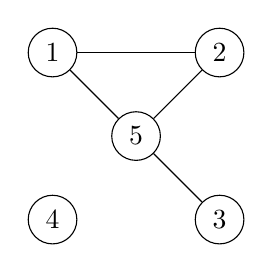
\begin{tikzpicture}[node distance={15mm}, main/.style = {draw, circle}, baseline=-8.0ex] 
    \node[main] (1) {$1$};
    \node[main] (2) [below right of=1] {$5$};
    \node[main] (3) [above right of=2] {$2$};
    \node[main] (4) [below left of=2] {$4$};
    \node[main] (5) [below right of=2] {$3$};

    \draw (1) -- (2);
    \draw (2) -- (3);

    \draw (2) -- (5);
    \draw (1) -- (3);
  \end{tikzpicture}

	\caption{Graf wraz z odpowiadającą mu macierzą sąsiedztwa. W tej macierzy 0 odpowiada brakowi krawędzi, a 1 odpowiada jej istnieniu.}
\end{figure}

Warto zauważyć nadmiarowość macierzy, gdzie każdej krawędzi w grafie odpowiadają dwie wartości. Ta nadmiarowość okazjonalnie pozwala na przyspieszenie obliczeń w zmodyfikowanej wersji macierzy sąsiedztwa używanej w naszym kodzie.
Modyfikacja metody macierzy sąsiedztwa polega na odejściu od zapisywania każdej liczby w macierzy jako osobnej wartości. Jako że zajmujemy się jedynie grafami prostymi i niekolorowanymi, to wartości w poszczególnych komórkach mogą wynosić jedynie 0 lub 1. W związku z tym wiersz macierzy można zapisać nie jako n wartości, a jako jedną wartość o odpowiedniej liczbie bitów. Ze względu na to, że największym grafem występującym w naszej pracy jest potencjalny graf 25 wierzchołkowy, 32 bitowa wartość jest wystarczająca żeby pomieścić wiersz macierzy reprezentujący wierzchołek dowolnego grafu który może zostać wygenerowany przez nasz program. 